\chapter[Dark Matter searches with neutrinos from the Sun]{Dark Matter searches\\ with neutrinos from the Sun}\label{chapter:dm_analysis}

\begin{chapquote}{Leo Tolstoy, \textit{Anna Karenina}}
	He stepped down, trying not to look long at her, as if she were the Sun, yet he saw her, like the Sun, even without looking.
\end{chapquote}

%Solar DM capture
The idea of detecting neutrino signals coming from the core of the Sun to probe \gls{dm} is not new. The main focus of these searches has usually been high-energy neutrinos originated from \gls{dm} annihilations into heavy particles \cite{Silk1985, Srednicki1986, Hagelin1986, Gaisser1986}. However, recent studies have proposed to look at the low-energy neutrino flux arising from the decay of light mesons at rest in the Sun \cite{Bernal2012, Rott2012, Rott2015, DUNE2021}, previously thought undetectable.

%
In this Chapter, I try to demonstrate the capability of \gls{dune} to constrain this kind of \gls{dm} scenarios. I use the neutrino fluxes arising from \gls{dm} annihilations in the core of the Sun to compute the projected limits that \gls{dune} would be able to set on the annihilation rates of \gls{dm} particles in the Sun and the \gls{dm} scattering cross sections.

\section{Gravitational capture of DM by the Sun}
\label{sec:dm_analysis_theory}

The Sun and the centre of the Earth are possible sources of \gls{dm} annihilations, specially interesting because of their proximity. Their gravitational attraction ensures the capture of \gls{dm} from the local halo through repeated scatterings of \gls{dm} particles crossing them. Only neutrinos produced from \gls{dm} annihilations can escape the dense interior of these objects. Therefore, neutrino telescopes are the most useful experimental layouts to pursue \gls{dm} searches from their cores.

The neutrino flux from \gls{dm} annihilations inside the Sun depends on the \gls{dm} capture rate, which is proportional to the \gls{dm} scattering cross section, and the annihilation rate, which is proportional to the velocity-averaged \gls{dm} annihilation cross section. The total number of \gls{dm} particles inside the Sun follows the Boltzmann equation \cite{Bernal2012}:
\begin{equation}\label{2.1}
	\frac{\mathrm{d} N_{DM}}{\mathrm{d} t} = C_{\odot} - A_{\odot} N_{DM}^{2},
\end{equation}
where $C_{\odot}$ and $A_{\odot}$ are the total Sun \gls{dm} capture and annihilation rates respectively. In this expression I neglected the evaporation term, proportional to $N_{DM}$, which only contribute for $m_{\mathrm{DM}}\lesssim 4$ GeV \cite{Busoni2013}. As the current threshold of neutrino telescopes is a few GeV, this region falls below the probed range but can be important in future low-energy projects like \gls{dune}.

This equation has an equilibrium solution:
\begin{equation}\label{2.2}
	N_{DM}^{eq} = \sqrt{\frac{C_{\odot}}{A_{\odot}}},
\end{equation}
which represents the amount of \gls{dm} inside the Sun if the capture and annihilation have reached equilibrium. As the Sun is approximately $4.6$ Gyr old \cite{Bahcall1995}, it is usually assumed that equilibrium has been achieved. Therefore, the anomalous neutrino flux from the Sun would only depend on the \gls{dm} scattering cross section, enabling us to set limits on this quantity. If one does not assume equilibrium, some assumptions on the \gls{dm} annihilation cross section are necessary to extract predictions from the neutrino signals.

A detailed discussion regarding the computation of the capture rates is given in App. \ref{sec:dm_analysis_capture_rates}.

\section{Neutrino flux from DM annihilations}
\label{sec:dm_analysis_flux}

When \gls{wimp}s annihilate inside the Sun a flux of high-energy neutrinos is expected from heavy quarks, gauge bosons and $\tau^{+}\tau^{-}$ final states, which decay before losing energy in the dense solar medium \cite{Rott2012}. These produce a continuous neutrino spectra up to $E_{\nu} \sim m_{\mathrm{DM}}$. In the case of direct annihilation into neutrinos, one would have a monochromatic flux with $E_{\nu} = m_{\mathrm{DM}}$. This kind of signal has been extensively studied  in the literature, allowing to put strong limits on the \gls{sd} \gls{wimp}-proton cross section for large $m_{\mathrm{DM}}$. However, the number of high-energy neutrinos per \gls{wimp} annihilation is small and the spectrum depends on the unknown final state. Moreover, although background rejection is easier for large $m_{\mathrm{DM}}$, neutrinos with $E_{\nu} \gtrsim 100 ~ \mathrm{GeV}$ are significantly attenuated by interactions in the Sun.

Nevertheless, most \gls{wimp} annihilation final states eventually produce a low-energy neutrino spectrum.  In this case one does not just consider the more massive final states but also annihilations into $e^{+}e^{-}$, $\mu^{+}\mu^{-}$ and light quarks \cite{Bernal2012}. In particular, light mesons would be produced and stopped in the dense medium, thus decaying at rest and producing a monoenergetic neutrino signal. The decay-at-rest of kaons will produce a $\nu_{\mu}$ flux with $E_{\nu} = 236 ~ \mathrm{MeV}$, while in the case of pions one would have $E_{\nu}  = 29.8 ~ \mathrm{MeV}$. In practice, only the $K^{+}$ and $\pi^{+}$ contribute to these signals, as the $K^{-}$ and $\pi^{-}$ are usually Coulomb-captured in an atomic orbit and get absorbed by the nucleus. There is also a low-energy neutrino signal coming from muon decays, which are produced in kaon or pion decays, leptonic decays of other hadrons and heavy leptons or even directly from \gls{wimp} annihilations. These can decay at rest and contribute to the previous low-energy neutrino flux with a well known spectrum below $52.8 ~ \mathrm{MeV}$.

These monoenergetic $\mathrm{MeV}$ neutrinos were previously considered undetectable but, due to the large yield, the known spectra and the modern advances in the detector technology, these low-energy neutrino flux can be a good probe of the \gls{sd} \gls{wimp}-proton cross section in the standard solar \gls{wimp} capture scenario, as it is sensitive to low \gls{wimp} masses and insensitive to the particular final state. A good place to look for these signals are next-generation neutrino experiments such as \gls{dune} \cite{DUNE2021}.

\section{Computing limits from solar neutrino fluxes}
\label{sec:dm_analysis_limits}

\begin{figure}[t]
	\centering
	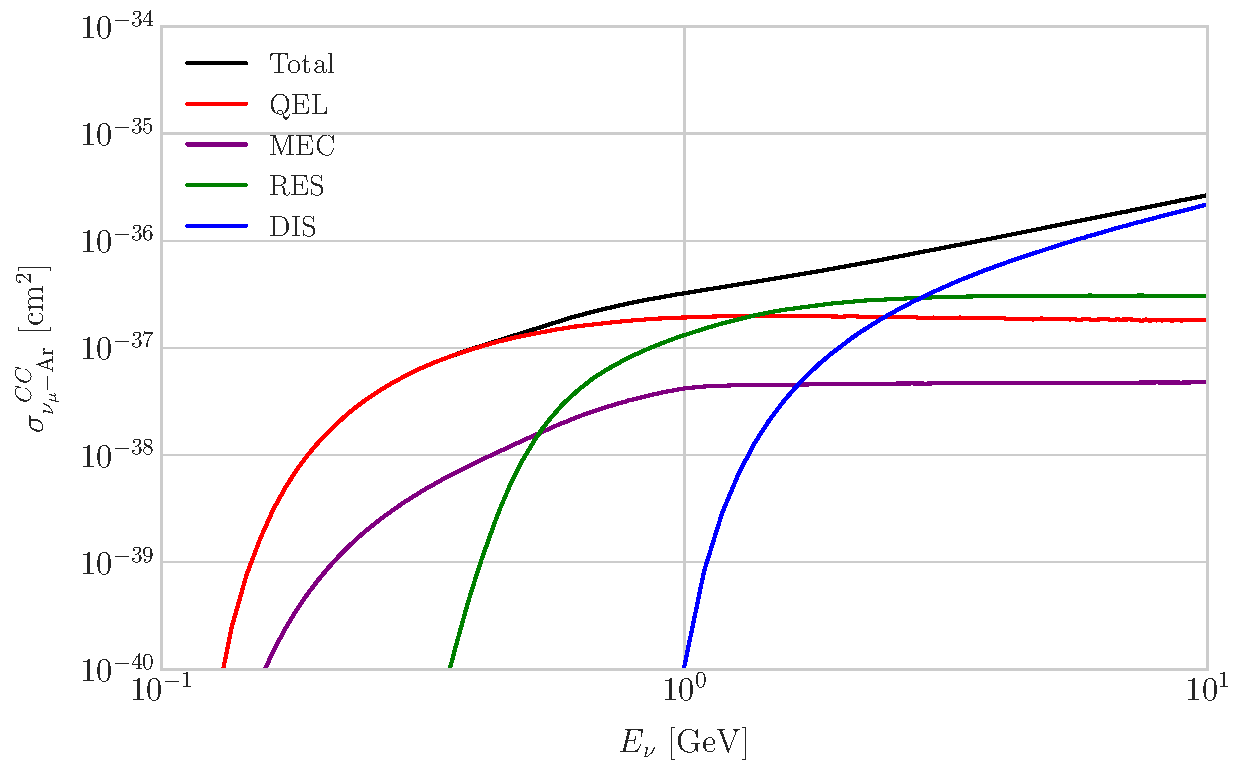
\includegraphics[width=0.9\linewidth]{Images/DM_Analysis/nu_Ar_xsection}
	\caption[\texttt{NuWro}-computed $\nu_{\mu}-\ce{^{40}Ar}$ charged-current scattering cross section as a function of the neutrino energy.]{\texttt{NuWro}-computed $\nu_{\mu}-\ce{^{40}Ar}$ charged-current scattering cross section as a function of the neutrino energy. The black line shows to the total cross section, whereas the others correspond to the different contributions (in red quasi-elastic scattering, in green resonant pion exchange, in blue deep inelastic scattering and in purple meson exchange current).}
	\label{fig:nu_Ar_xsection}
\end{figure}

The first step to use these fluxes to search for \gls{dm} in the Sun is to determine the expected number of atmospheric background events. For a given exposure, after directionality selection has been applied, this can be written as:
\begin{equation}\label{4.1}
	N_{B} = \eta_{B} \int \mathrm{d}\Omega \int_{E_{min}}^{E_{max}} \mathrm{d}E_{\nu} \ \frac{\mathrm{d}^{2}\Phi_{atm}^{\mu}}{\mathrm{d}E_{\nu} \mathrm{d}\Omega} \times \left(A_{eff}^{(\mu)}(E_{\nu}) T\right),
\end{equation}
where $\eta_{B}$ is the background efficiency, $E_{min}$ and $E_{max}$ the minimum and maximum energies to integrate over, $\mathrm{d}^{2}\Phi_{atm}^{\mu} / \mathrm{d}E_{\nu} \mathrm{d}\Omega$ the differential flux of atmospheric muon neutrinos, $A_{eff}^{(\mu)}$ is the effective area of \gls{dune} to muon neutrinos, and $T$ is the exposure time. The effective area can be expressed as the product of the neutrino-nucleus scattering cross section and the number of nuclei in the fiducial volume of the detector. This way, for \gls{dune} we have:
\begin{equation}\label{4.2}
	A_{eff}^{(\mu)}(E_{\nu}) = (6.0 \times 10^{-10} \ \mathrm{m}^{2}) \left(\frac{\sigma_{\nu - \mathrm{Ar}}^{(\mu)}(E_{\nu})}{10^{-38} \ \mathrm{cm}^{2}}\right) \left(\frac{M_{target}}{40 \ \mathrm{kT}}\right),
\end{equation}
where $\sigma_{\nu - \mathrm{Ar}}^{(\mu)}$ is the $\nu_{\mu}-\ce{^{40}Ar}$ charged-current scattering cross section. In Fig. \ref{fig:nu_Ar_xsection} I show the computed value of the cross section as a function of the neutrino energy $E_{\nu}$, in the range of interest both for the atmospheric background and signal events. It was computed using the \texttt{NuWro} Monte Carlo neutrino event generator \cite{Golan2012}, including the \gls{qe} (red line), \gls{mec} (purple line), \gls{res} (green line), and \gls{dis} (blue line) \gls{cc} contributions.

The background rejection will depend on the resolution of the detector and the selection one applies on the events. A geometry argument can be used to estimate the maximum background rejection one can achieve in this case, considering one can efficiently discriminate all events coming from a direction different from that of the Sun. In that case, the optimal background efficiency will simply be the relative angular coverage of the Sun. Taking the angular diameter of the Sun as seen from the Earth to be $0.5^{\circ}$, one obtains:
\begin{equation}\label{4.3}
	\eta_{B}^{(opt)} \approx \frac{\pi \left(\frac{0.5}{2}\right)^{2}}{360 \times 180} \simeq 3.03 \times 10^{-6}.
\end{equation}
This value gives an optimistic estimate of the number of background events. However, it can be regarded as an upper limit, as it represents the best case scenario.

In Fig. \ref{fig:homestake_fluxes} I show the fluxes of atmospheric neutrinos at the Homestake mine during solar minimum, taken from Ref. \cite{Honda2015}. The values are averaged over the two angular directions. In blue I have the flux of muon neutrinos while in red I indicate the flux of electron neutrinos. Additionally, the dashed lines correspond to both antineutrino species.

Using these values for the muon neutrino and the corresponding total \gls{cc} cross section, one can compute the total number of expected background events by integrating over the given energy range. For this I choose the energy range for the \gls{dune} \gls{fd} specified in \cite{DUNE2020TDR2}, $E_{min} = 10^{-1} \ \mathrm{GeV}$ and $E_{max} = 10 \ \mathrm{GeV}$. Taking all these into account, I find the total number of background events to be:
\begin{equation}\label{4.4}
	N_{B} \simeq  \eta_{B} \times \left(3.827 \times 10^{4}\right) \times \left(\frac{\mathrm{exposure}}{400 \ \mathrm{kT \ yr}}\right).
\end{equation}

\begin{figure}[t]
	\centering
	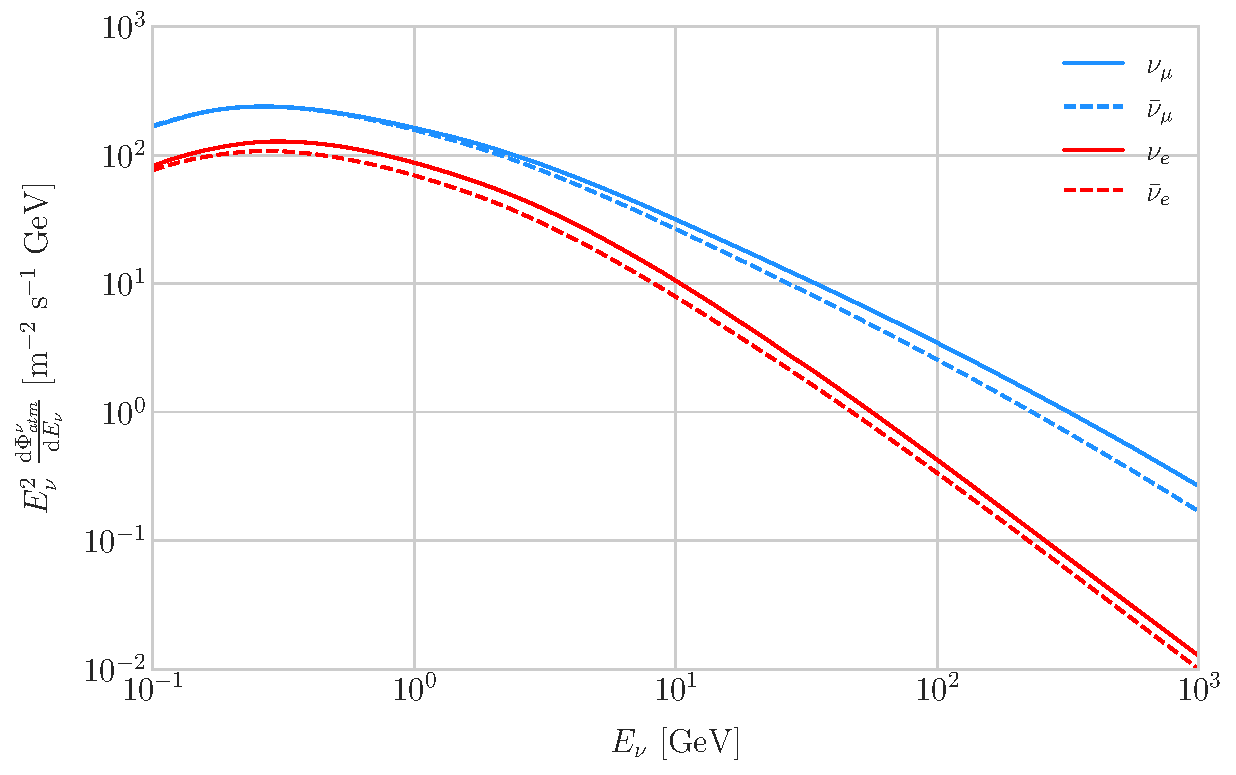
\includegraphics[width=0.9\linewidth]{Images/DM_Analysis/homestake_fluxes}
	\caption[Expected atmospheric neutrino flux as a function of the neutrino energy $E_{\nu}$ at Homestake at solar minimum.]{Expected atmospheric neutrino flux as a function of the neutrino energy $E_{\nu}$ at Homestake at solar minimum, taken from Ref. \cite{Honda2015}. The blue solid (dashed) line correspond to muon neutrinos (antineutrinos) and the red solid (dashed) line correspond to electron neutrinos (antineutrinos).}
	\label{fig:homestake_fluxes}
\end{figure}

To estimate the sensitivity of \gls{dune} to this kind of signals, one can consider a hypothetical data set where the number of observed neutrinos is taken to be the expected number of background events rounded to the nearest integer, $N_{obs} = \mathrm{round}(N_{B})$ \cite{Cowan2010}. Now, if I assume that the number of signal and background events seen by \gls{dune} are given by Poisson distributions with means equal to the expected number of signal and background events, $N_{S}$ and $N_{B}$, one can denote by $N_{S}^{90}$ to the number of expected signal events such that the probability of having an experimental run with a number of events greater than $N_{obs}$ is $90\%$. This number can be obtained as the numerical solution to the equation:
\begin{equation}\label{4.5}
	1 - \frac{\Gamma\left(N_{obs}+1, N_{S}^{90}+N_{B}\right)}{N_{obs}!} = 0.9,
\end{equation}
where $\Gamma(x,y)$ is the upper incomplete gamma function.

The number of signal events is related to the neutrino flux from \gls{dm} annihilations in a similar way as the background events to the atmospheric neutrino flux. In this case I have:
\begin{equation}\label{4.6}
	N_{S} = \eta_{S} \ \Gamma_{A}^{eq} \int_{z_{min}}^{z_{max}} \mathrm{d}z \ \frac{\mathrm{d}N_{\nu}}{\mathrm{d}A \mathrm{d}N_{A} \mathrm{d}z}  \times \left(A_{eff}^{\mu}(z) T\right),
\end{equation}
where $\eta_{S}$ is the signal efficiency, $\Gamma_{A}^{eq}$ is the total annihilation rate of \gls{dm} particles at equilibrium, $\Gamma_{A}^{eq} = A_{\odot} \left(N_{DM}^{eq}\right)^{2}$, $z_{min}$ and $z_{max}$ the minimum and maximum relative energies to integrate over (given by $z_{min, max} = E_{min, max}/m_{\mathrm{DM}}$ for each $m_{\mathrm{DM}}$) and $\mathrm{d}N_{\nu}/\mathrm{d}A \mathrm{d}N_{A} \mathrm{d}z$ the muon neutrino flux per \gls{dm} annihilation in the Sun.

Having obtained $N_{S}^{90}$ one can use the relation in Eq. (\ref{4.6}) to compute $\Gamma_{A}^{eq,90}$ for different values of the \gls{dm} mass. Then, I can directly translate those values into the projected sensitivities for \gls{dune} to the \gls{dm} scattering cross sections, for a given exposure. The relation between the annihilation rate and the \gls{dm}-nucleon cross section comes from the equilibrium condition through the solar \gls{dm} capture rate, discussed above.

\section{High energy DM neutrino signals}
\label{sec:dm_analysis_high_e_nu}

\begin{figure}[t]
	\centering
	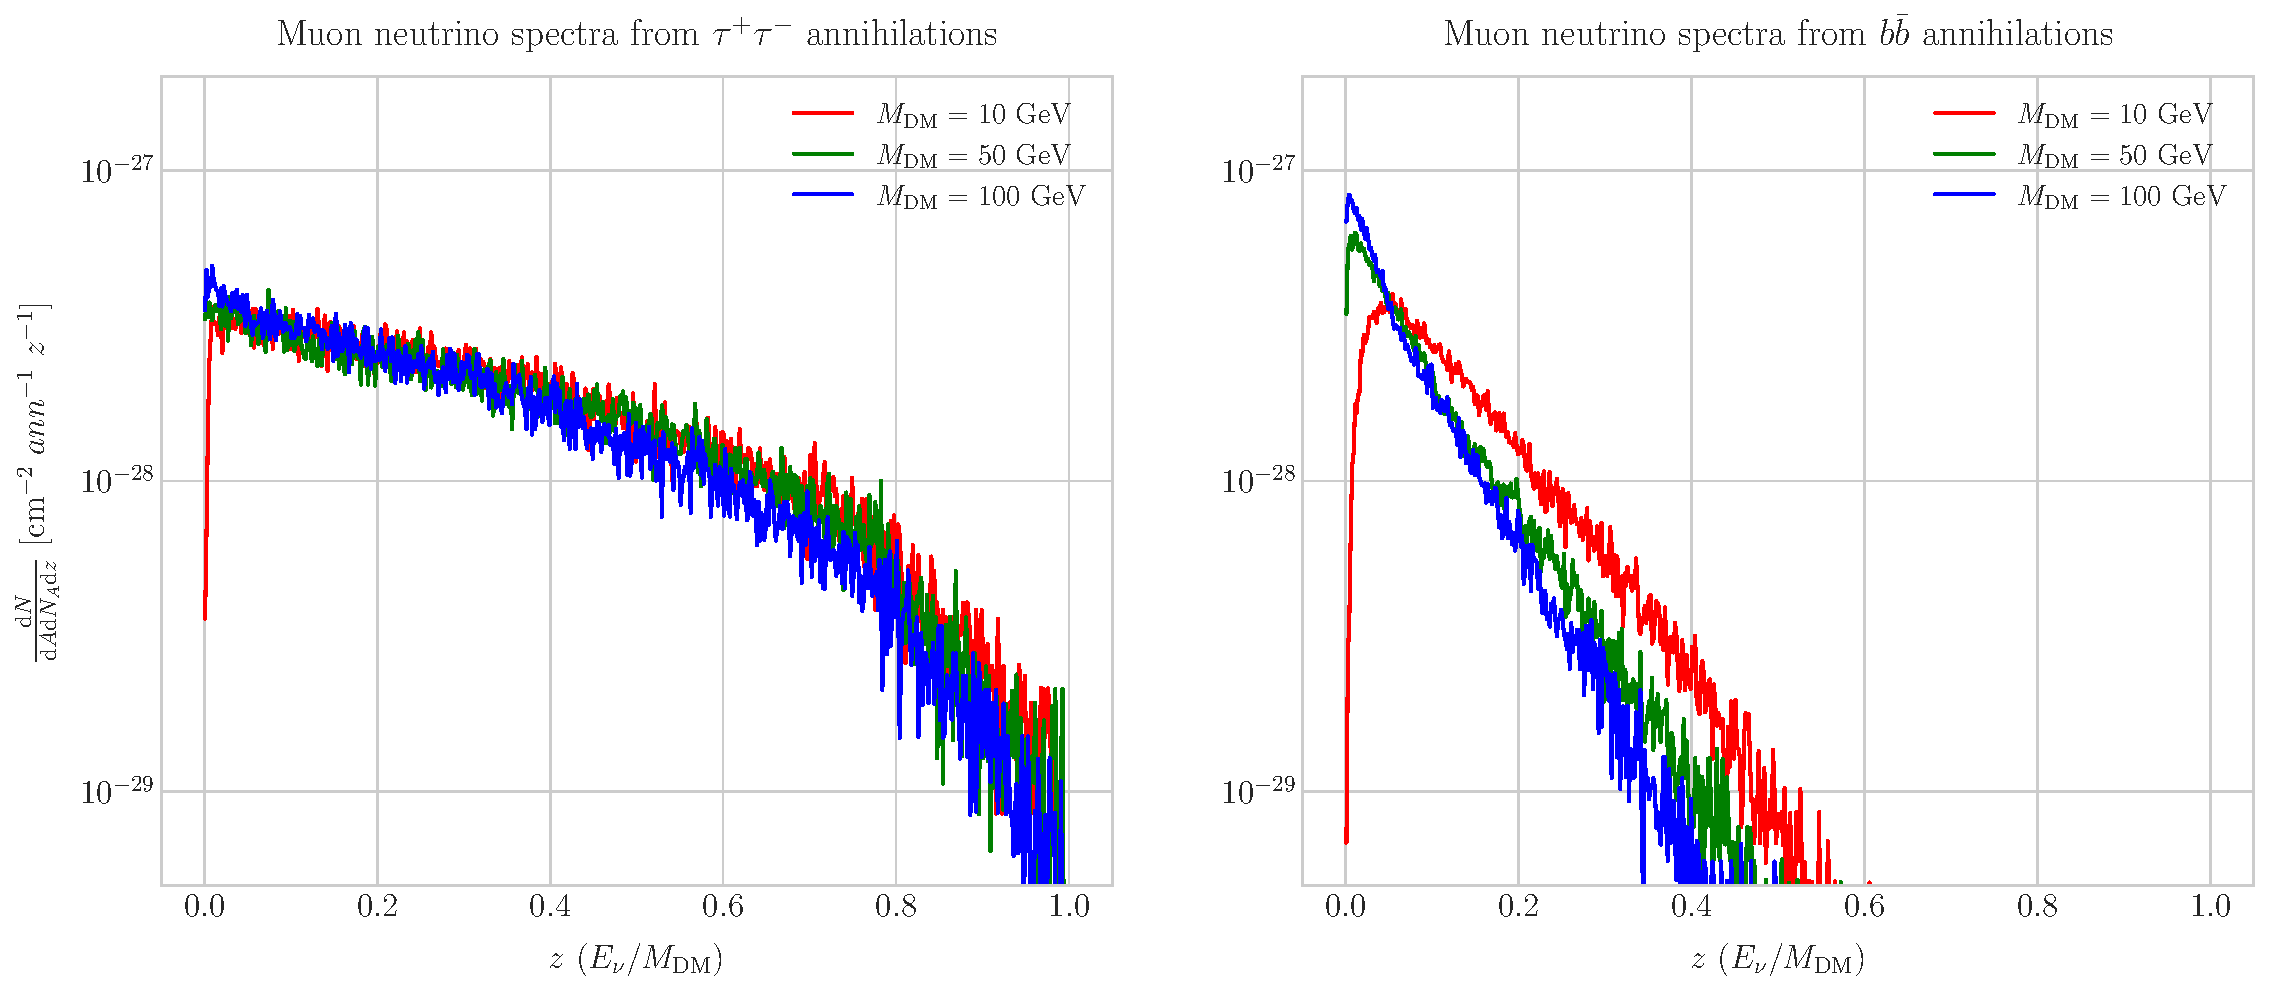
\includegraphics[width=1\linewidth]{Images/DM_Analysis/solardm_nu_mu_spectra.pdf}
	\caption[Computed spectra of muon neutrinos at the \gls{dune} \gls{fd} site from $\tau^{+} \tau^{-}$ and $b\bar{b}$ annihilations in the Sun for different \gls{dm} masses.]{Computed spectra of muon neutrinos at the \gls{dune} \gls{fd} site from $\tau^{+} \tau^{-}$ (left panel) and $b\bar{b}$ (right panel) annihilations in the Sun for the \gls{dm} masses $m_{\mathrm{DM}} = 10 \ \mathrm{GeV}$ (red line), $50 \ \mathrm{GeV}$ (green line) and $100 \ \mathrm{GeV}$ (blue line), plotted in relative energy units.}
	\label{fig:solardm_nu_mu_spectra}
\end{figure}

To make accurate estimates of the capability of the \gls{dune} \gls{fd} to constrain the parameter space of the \gls{dm} using solar neutrino fluxes, I need to account for the detector resolution effects and the topologies of the different signatures. As a starting point, I focus on specific \gls{dm} self-annihilation channels. For the case of \gls{dune}, the relevant ones are mainly the hard channels $\tau^{+} \tau^{-}$ and $\nu \bar{\nu}$ and the soft channel $b\bar{b}$. These are the annihilation channels open for relatively low mass \gls{wimp}s that will actually give neutrino fluxes. Other channels, like $W^{+} W^{-}$ and $ZZ$, are open for more massive \gls{wimp}s. However, those will produce a higher energy neutrino flux that will be out of reach for \gls{dune} (the maximum neutrino energy for a detector like the \gls{dune} \gls{fd} is taken to be $E_{max} = 10 \ \mathrm{GeV}$).

In Fig. \ref{fig:solardm_nu_mu_spectra} I show the muon neutrino spectra at the \gls{dune} \gls{fd} location (44$^{\circ} $ 20' N, 103$^{\circ} $ 45' W) generated with \texttt{WimpSim} \cite{WimpSim} from $\tau^{+} \tau^{-}$ (left panel) and $b\bar{b}$ (right panel) annihilations in the core of the Sun, for different \gls{dm} masses. Here, one can clearly see the meaning of the previous distinction between hard and soft channels. For the same \gls{dm} mass value, the muon neutrino spectrum from the $\tau^{+} \tau^{-}$ channel is more flat and reaches higher energies than the one from the $b\bar{b}$ channel, which drops faster.

In this case, I prepared two sets of samples, one for $\tau^{+} \tau^{-}$ and the other for $b\bar{b}$, for \gls{dm} masses in the range from $5$ to $100 \ \mathrm{GeV}$ (for $b\bar{b}$ the first mass point I consider is $7.5 \ \mathrm{GeV}$, as this annihilation channel is not kinematically allowed for a \gls{wimp} with $m_{\mathrm{DM}}=5 \ \mathrm{GeV}$). For each channel and mass value, I generate $10^{5}$ neutrino events in \texttt{WimpSim}, that I then pass to \texttt{NuWro} which simulates the neutrino interaction with the argon.

\texttt{WimpSim} outputs both a flux file and an event list for the specified channel and mass value. The directions of these events are given in terms of the azimuth and altitude angles viewed from the specified location, so first I need to convert these into the \gls{dune} \gls{fd} coordinates. Once I have done this, each event is used as input for \texttt{NuWro}. I restrict the event generation to charged current interactions, but I allow all the different contributions to the \gls{cc} cross section, i.e. \gls{qe}, \gls{mec}, \gls{res}, and \gls{dis}. I exclusively take into account the \gls{cc} contribution because I am only interested in final states with charged leptons, as we have better chances of reconstructing the kinematics of these events.

\begin{figure}[t]
	\centering
	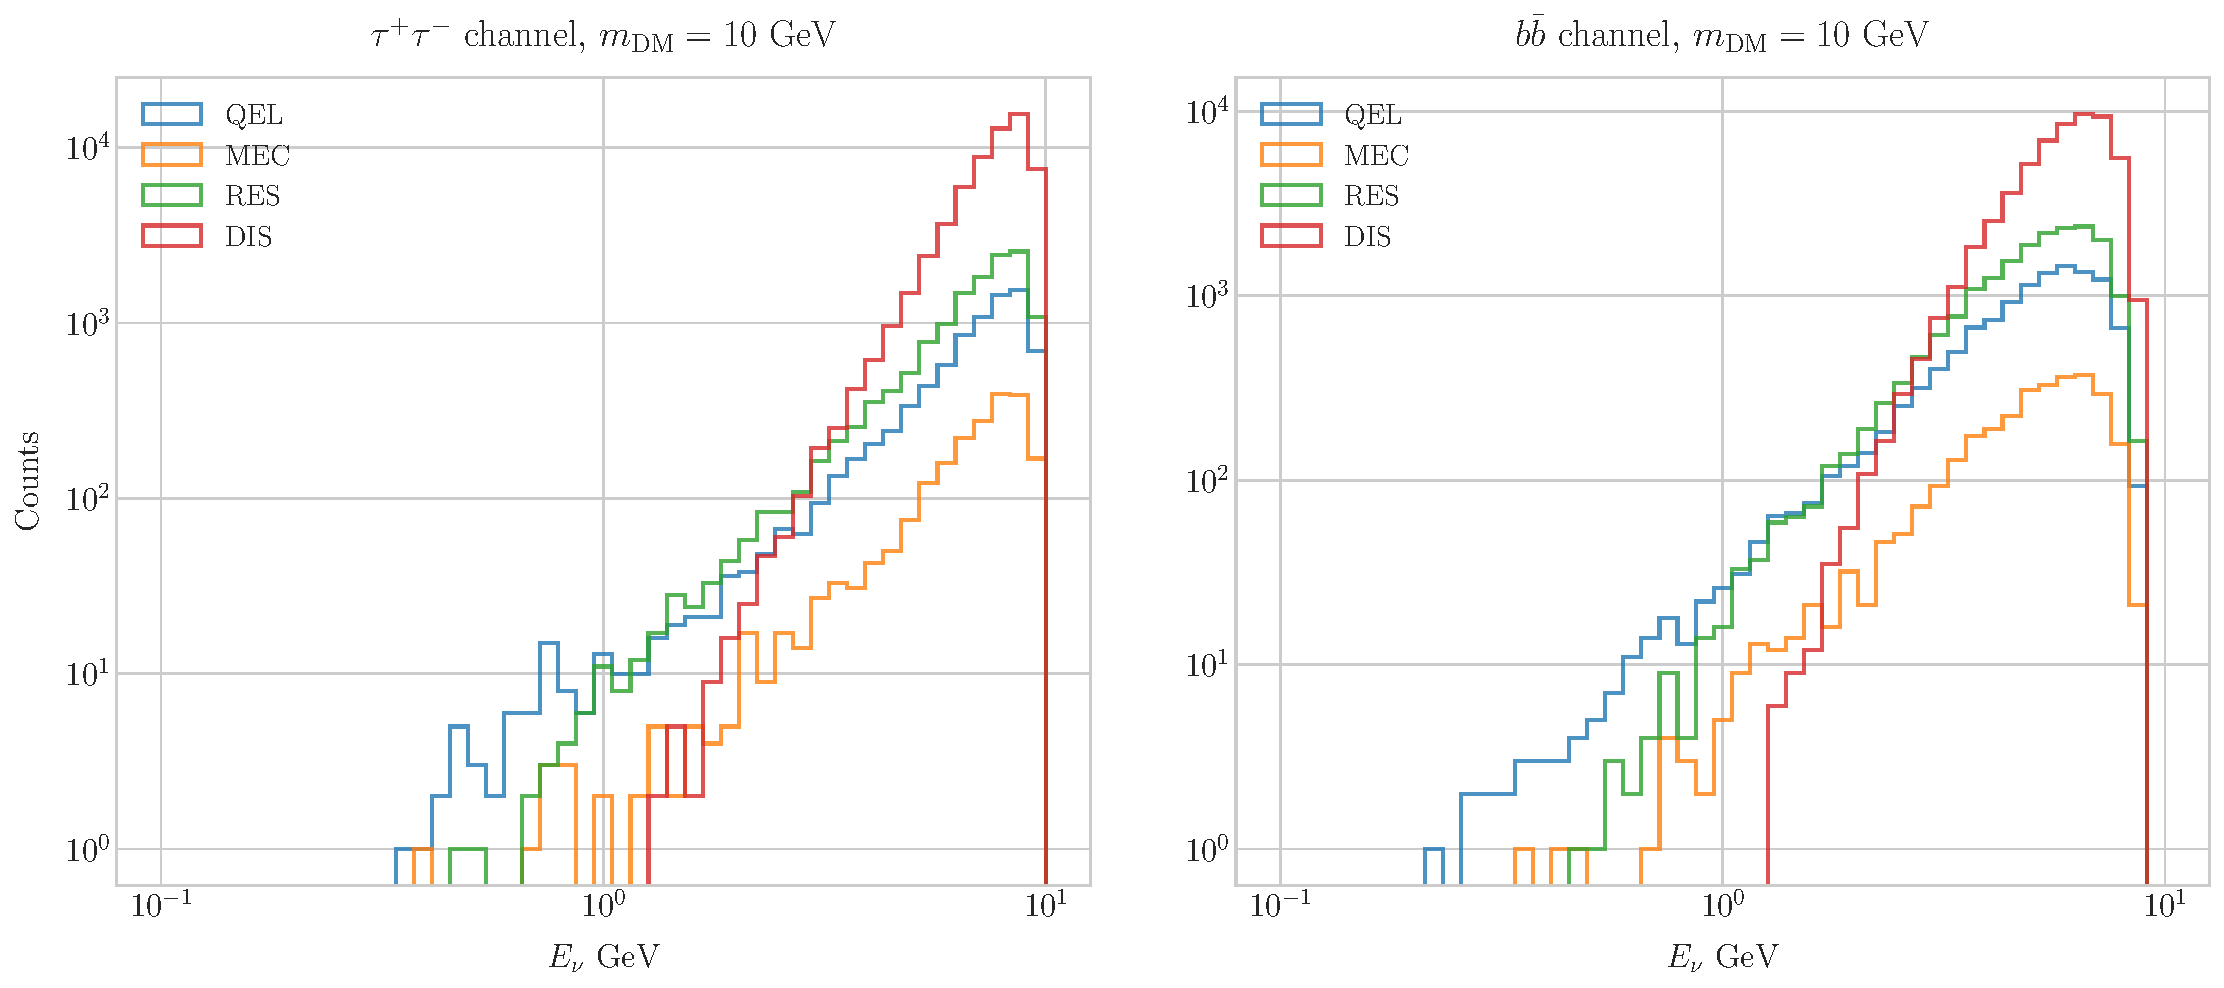
\includegraphics[width=1\linewidth]{Images/DM_Analysis/solardm_nu_mu_interactions.pdf}
	\caption[Distribution of the muon neutrino energies from the $\tau^{+} \tau^{-}$ and $b\bar{b}$ annihilation channels.]{Distribution of the muon neutrino energies from the $\tau^{+} \tau^{-}$ (left panel) and $b\bar{b}$ (right panel) annihilation channels, for $m_{\mathrm{DM}} = 10 \ \mathrm{GeV}$, separated by \gls{cc} interaction type: \gls{qe} (blue), \gls{mec} (orange), \gls{res} (green) and \gls{dis} (red).}
	\label{fig:solardm_nu_mu_interactions}
\end{figure}

For the atmospheric fluxes I follow a similar procedure, using the fluxes binned in azimuth and altitude angles. This way, I transform these to \gls{dune} coordinates and process the fluxes for each bin separated with \texttt{NuWro}, generating a total of $10^{5}$ background events.

At this point, I have two sets of neutrino signal events with different energies and final states. In Fig. \ref{fig:solardm_nu_mu_interactions} one can see the distribution of the muon neutrino energies for the case $m_{\mathrm{DM}} = 10 \ \mathrm{GeV}$, both for the $\tau^{+} \tau^{-}$ (left panel) and $b\bar{b}$ (right panel) channels, separated by interaction. One can clearly see that there are various energy regimes where different interaction types dominate. This leads to a plurality of event topologies, therefore making it difficult to implement a general approach to the selection of events in detriment of the background. As a way to proceed, I decided to focus on a subset of the samples, based on the different interaction modes and contents of the final state. Thus, I consider a \gls{cc} \gls{dis} sample and a single proton \gls{cc} \gls{qe} sample.

\begin{figure}[t]
	\centering
	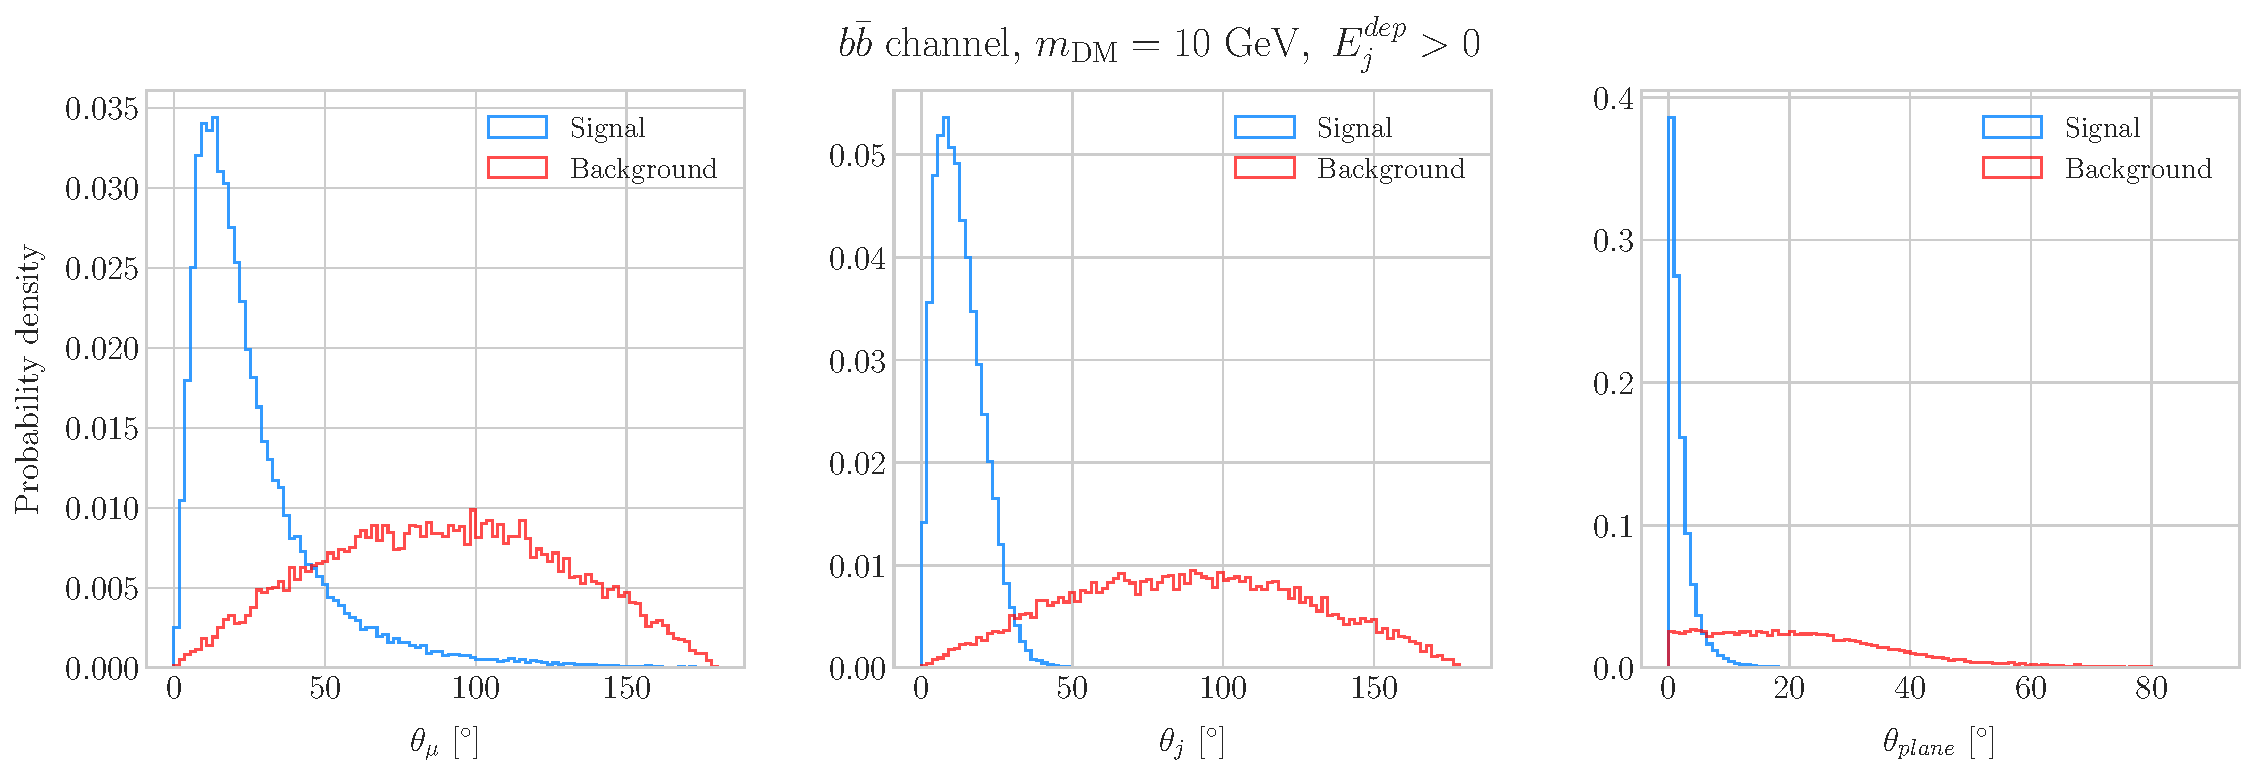
\includegraphics[width=0.95\linewidth]{Images/DM_Analysis/solardm_bb_100_dis_angular_dists.pdf}
	\caption[Angular distributions for the $b\bar{b}$ \gls{dis} sample with $m_{\mathrm{DM}} = 10 \ \mathrm{GeV}$ and the atmospheric background.]{Distributions of $\theta_{\mu}$ (left panel), $\theta_{j}$ (central panel) and $\theta_{plane}$ (right panel) for the $b\bar{b}$ sample with $m_{\mathrm{DM}} = 10 \ \mathrm{GeV}$ (blue) and the atmospheric background (red).}
	\label{fig:solardm_bb_100_dis_angular_dists}
\end{figure}

\subsection{DIS-like events}

To begin with, I consider the high energy part of the neutrino spectrum. In this region \gls{dis} events dominate, i.e. interactions of the form $\nu_{\mu} + q_{d}(\bar{q}_{u}) \rightarrow \mu^{-} + q_{u}(\bar{q}_{d})$. Therefore, our final states will contain a muon and a hadronic jet from the fragmentation of the outgoing quark. As all these events have $E_{\nu} \gtrsim 1 \ \mathrm{GeV}$ the momentum transfer to the remnant nucleus is negligible. For this reason, the neutrino energy can be effectively reconstructed just taking into account the momenta of the muon and the jet. This technique was successfully used in Ref. \cite{Rott2019} to select monoenergetic \gls{dm} solar neutrino events from the $\nu \bar{\nu}$ annihilation channels.

Using momentum conservation one sees that the plane generated by the momenta of the muon and the jet also needs to contain the momentum of the neutrino. As we are interested in neutrinos coming from the Sun, the direction of the neutrino can be regarded as known beforehand. This will allow us to define the angle of the outgoing muon and jet with respect to the incoming neutrino for each event. Moreover, one can also use that information to reject poorly reconstructed jets, checking for deviations of these from the momentum conservation plane.

To account for the limited angular resolution of the detector, I smeared the momenta of the muons and hadrons. In a \gls{lartpc} muons are expected to be tracked with high precision, therefore I take the associated angular resolution to be $1^{\circ}$. In the case of jets, it is expected that for the hadrons dominating the cascade a detector like the \gls{dune} \gls{fd} will have an angular resolution between $1^{\circ}$ to $5^{\circ}$ \cite{DUNE2020TDR2}, so I take the latter for a more conservative estimate.

As a first step, I perform a truth-level pre-selection on the \gls{dis} events, requiring the \gls{fsi} particles to have kinetic energies above the detection thresholds of \gls{dune}. For muons and photons the specified threshold energy is $30 ~ \mathrm{MeV}$, for charged pions $100 ~ \mathrm{MeV}$, and for other hadrons $50 ~ \mathrm{MeV}$ \cite{DUNE2020TDR2}. This way, I will drop an event if the outgoing muon has an energy lower than the required threshold. For the case of hadrons and photons, I only require to have at least one particle above the energy threshold, so then one can compute the jet momentum using the (smeared) momenta of the $N$ particles above threshold as:
\begin{equation}
	\vec{p}_{j} = \sum_{i=1}^{N} \vec{p}_{i}.
\end{equation}

\begin{figure}[t]
	\centering
	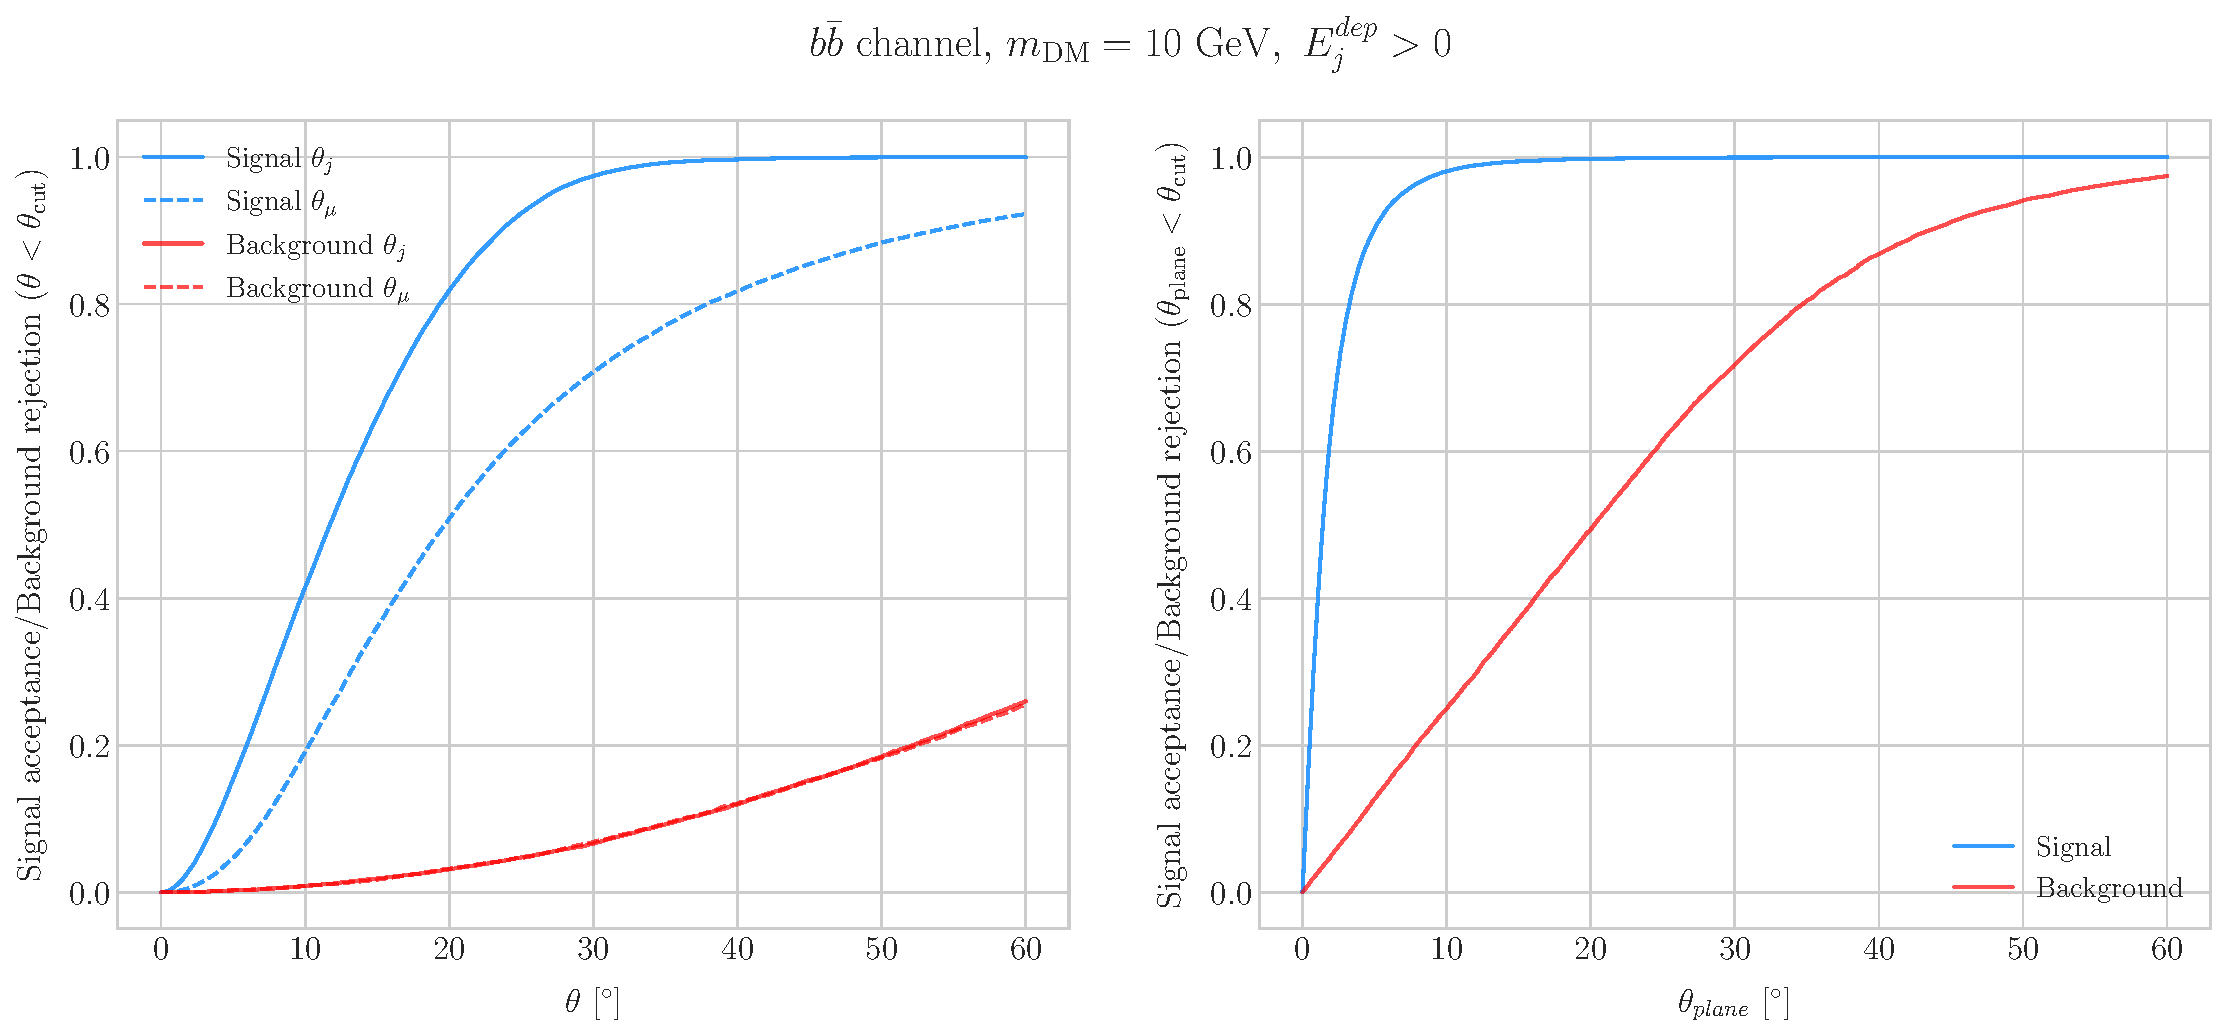
\includegraphics[width=0.95\linewidth]{Images/DM_Analysis/solardm_bb_100_dis_angular_cuts.pdf}
	\caption[Signal efficiency and background rejection for the $b\bar{b}$ sample with $m_{\mathrm{DM}} = 10 \ \mathrm{GeV}$ as a function of the angular cuts.]{Left panel: signal efficiencies (blue lines) and background rejections (red lines) for events passing the cuts $\theta < \theta_{cut}$ for the jet (solid lines) and muon (dashed lines) angles. Right panel: signal efficiency (blue line) and background rejection (red line) for events passing the cut $\theta_{plane} < \theta_{cut}$ for the momentum conservation plane deviation.}
	\label{fig:solardm_bb_100_dis_angular_cuts}
\end{figure}

Additionally, I also estimate the deposited hadronic energy as:
\begin{equation}
	E_{j}^{dep} = m_{^{39}\mathrm{Ar}} - m_{^{40}\mathrm{Ar}} + \sum_{i=1}^{N} \sqrt{|\vec{p}_{i}|^{2} + m_{i}^{2}}.
\end{equation}
This quantity is useful to select events with enough hadronic visible energy in the detector. For events where most of the hadronic energy is scattered across plenty of hadrons with individual energies below the detection threshold, this estimation will give $E_{j}^{dep} \leq 0$. In these cases it is expected that the jet momentum is poorly reconstructed, and therefore I require events to pass the cut $E_{j}^{dep} > 0$.

For the events passing the pre-selection, I can compute the angles for the muon and jet with respect to the incoming neutrino as:
\begin{align}
	\mathrm{cos} \ \theta_{\mu} &= \hat{p}_{\nu} \cdot \hat{p}_{\mu},\\
	\mathrm{cos} \ \theta_{j} &= \hat{p}_{\nu} \cdot \hat{p}_{j},
\end{align}
and the deviation from the momentum conservation plane as:
\begin{equation}
	\mathrm{sin} \ \theta_{plane} = \left|\frac{\hat{p}_{\mu} \cross \hat{p}_{\nu}}{|\hat{p}_{\mu} \cross \hat{p}_{\nu}|} \cdot \hat{p}_{j}\right|.
\end{equation}

In Fig. \ref{fig:solardm_bb_100_dis_angular_dists} I show some distributions of these quantities for the case of the $b\bar{b}$ sample with $m_{\mathrm{DM}} = 10 \ \mathrm{GeV}$ (blue histograms) and for the atmospheric backgrounds (red). To select the atmospheric events I follow the same criteria as for the signal events. However, because in the signal case I use the true direction of the neutrino as input, as it should be that of the Sun at that time and therefore known, in the atmospheric case I use a set of solar positions as the ansatz for the neutrino direction. From the distributions, one can see that the muon and the jet for the signal events are predominantly forward, and also that the deviations from the momentum conservation plane are peaked at zero, as one should expect.

\begin{figure}[t]
	\centering
	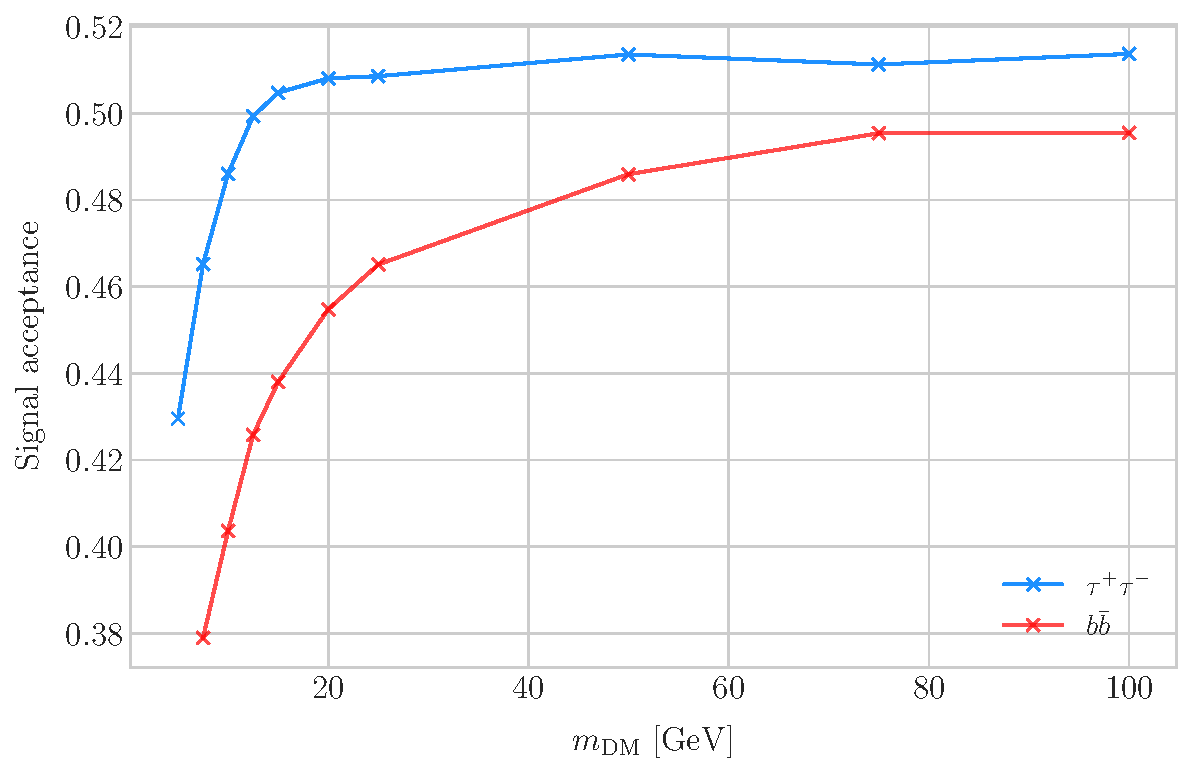
\includegraphics[width=0.9\linewidth]{Images/DM_Analysis/solardm_dis_signal_acceptance.pdf}
	\caption[Signal efficiencies for the $\tau^{+} \tau^{-}$ and $b\bar{b}$ \gls{dis} samples as functions of the \gls{dm} mass.]{Signal efficiencies for the $\tau^{+} \tau^{-}$ (blue line) and $b\bar{b}$ (red line) \gls{dis} samples as functions of the \gls{dm} mass, $m_{\mathrm{DM}}$, obtained by applying the optimal angular cuts $\theta_{\mu} < 27^{\circ}$, $4^{\circ} < \theta_{j} < 26^{\circ}$ and $\theta_{plane} < 3.5^{\circ}$.}
	\label{fig:solardm_dis_efficiency}
\end{figure}

Now, I can start applying a set of cuts to maximise our signal selection efficiency, while at the same time I try to minimise the amount of atmospheric background events passing the selection. To this end, I need to find some lower and upper cuts for $\theta_{j}$ and $\theta_{\mu}$ and an upper bound for $\theta_{plane}$. In Fig. \ref{fig:solardm_bb_100_dis_angular_cuts} I show how upper bound cuts in the different angular variables affect the signal efficiency (blue lines) and the background rejection (red lines). Notice that the signal efficiency behaves in quite a different way when I apply cuts in the jet and the muon angles. On the contrary, the cuts on both variables have a similar effect on the background rejection.

In order to obtain the optimal set of cuts, I perform a multidimensional scan. I do this separately for the $\tau^{+} \tau^{-}$ and the $b\bar{b}$ samples. For each case, I scan the possible cuts for every mass point and then I take the mean value of the signal efficiency for each configuration, to get the mean efficiency for each set of cuts. I do a similar scan for the atmospheric sample independently. Then, I take the sets of cuts such that the background rejection achieved is greater than $99.8\%$ and search for the one which maximises the $\tau^{+} \tau^{-}$ and $b\bar{b}$ sample mean efficiencies. Keeping a high background rejection at expenses of the signal efficiency is necessary, as this search is dominated by the background.

I found that with the cuts $\theta_{\mu} < 27^{\circ}$, $4^{\circ} < \theta_{j} < 26^{\circ}$ and $\theta_{plane} < 3.5^{\circ}$ I get a background rejection of $99.80\%$ while achieving a $49.40\%$ and $44.92\%$ mean signal efficiencies for the $\tau^{+} \tau^{-}$ and $b\bar{b}$ signals, respectively.

In Fig. \ref{fig:solardm_dis_efficiency} I show the signal efficiencies as a function of the \gls{dm} mass for the $\tau^{+} \tau^{-}$ (blue line) and the $b\bar{b}$ (red line) \gls{dis} events, after applying the cuts discussed above, as well as the energy thresholds and hadronic visible energy pre-selections. One can see that the efficiency grows with the mass, as annihilations of more massive \gls{dm} particles will produce a neutrino spectrum centered at higher energies. This makes it easier to separate the signal from the atmospheric background, which peaks at lower energies. Notice also that the efficiency is higher for the $\tau^{+} \tau^{-}$ case at every mass point, as in general this channel produces neutrinos at higher energies than the corresponding $b\bar{b}$ channel.

\begin{figure}[t]
	\centering
	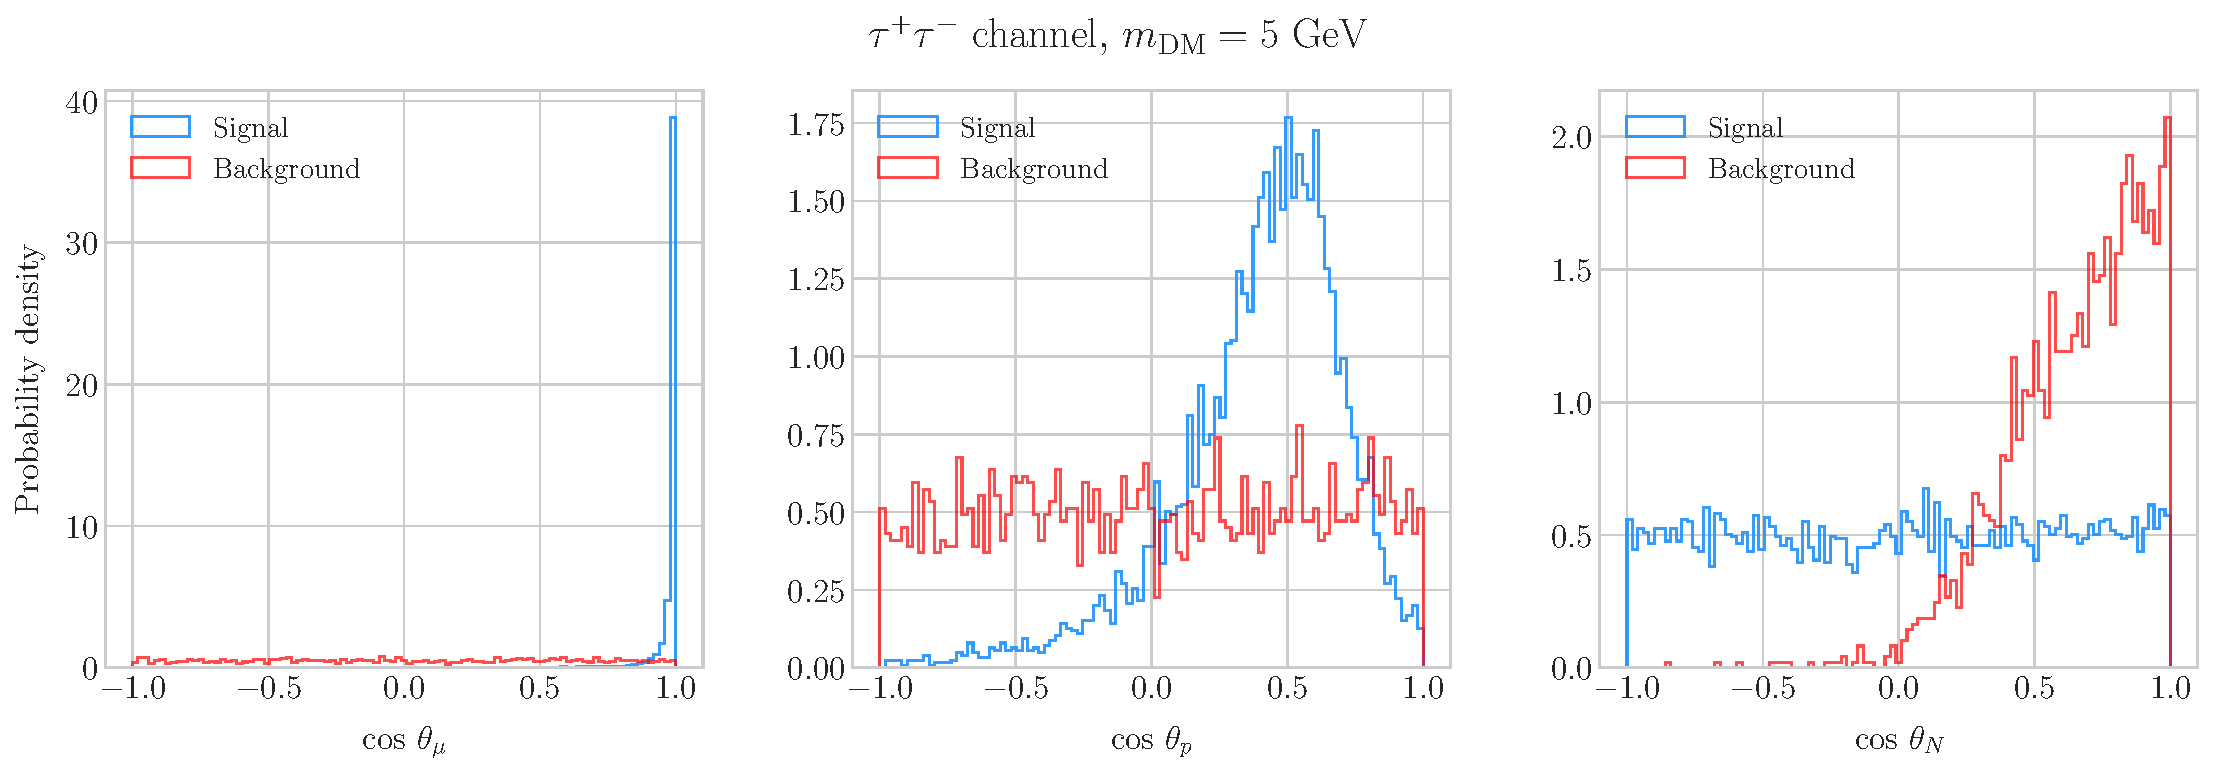
\includegraphics[width=0.95\linewidth]{Images/DM_Analysis/solardm_tau_5_qel_angular_dists.pdf}
	\caption[Angular distributions for the $\tau^{+}\tau^{-}$ \gls{qe} sample with $m_{\mathrm{DM}} = 5 \ \mathrm{GeV}$ and the atmospheric background.]{Distributions of $\mathrm{cos} \ \theta_{\mu}$ (left panel), $\mathrm{cos} \ \theta_{p}$ (central panel) and $\mathrm{cos} \ \theta_{N}$ (right panel) for the $\tau^{+}\tau^{-}$ \gls{qe} sample with $m_{\mathrm{DM}} = 5 \ \mathrm{GeV}$ (blue) and the atmospheric background (red).}
	\label{fig:solardm_tau_5_qel_angular_dists}
\end{figure}

\subsection{Single proton QE-like events}

Now, one can try to explore the low energy tail of the neutrino energy distributions. This regime is dominated by the \gls{qe} interactions, i.e. events of the type $\nu_{\mu} + n \rightarrow \mu^{-} + p$. The topology of these is very different from that of the \gls{dis} events, having typically just a muon and one proton in the final state. I will follow a similar treatment to that in Ref. \cite{DUNE2021} for the neutrinos from the $K^{+}$ decays at rest. However, the events at hand have higher energies and are not monochromatic.

In this case the momentum transfer to the remnant nucleus can be reconstructed from the kinematics of the \gls{fsi} particles. This can be important for events with $E_{\nu} \leq 1 ~ \mathrm{GeV}$. Therefore, I do not make the approximation I did before and assume that the momentum of the muon and the proton will give an adequate estimation of the reconstructed neutrino energy.

As before, I can take the direction of the incoming neutrino as known. That way, one can estimate the energy of the neutrino as:
\begin{equation}\label{6.6}
	E_{\nu}^{reco} = E_{\mu} + E_{p} + m_{^{39}\mathrm{Ar}} - m_{^{40}\mathrm{Ar}},
\end{equation}
and using momentum conservation I can write the momentum of the remnant nucleus as:
\begin{equation}\label{6.7}
	\vec{p}_{N} = \hat{p}_{\nu} \left(E_{\mu} + E_{p} + m_{^{39}\mathrm{Ar}} - m_{^{40}\mathrm{Ar}}\right) - \vec{p}_{\mu} - \vec{p}_{p}.
\end{equation}

As in the previous case, I need to drop the events where the muon or the proton fall below the kinetic energy detection threshold \cite{DUNE2020TDR2}. Also, I again apply a smearing to the momenta of the particles, $1\%$ for muons and $5\%$ for protons.

\begin{figure}[t]
	\centering
	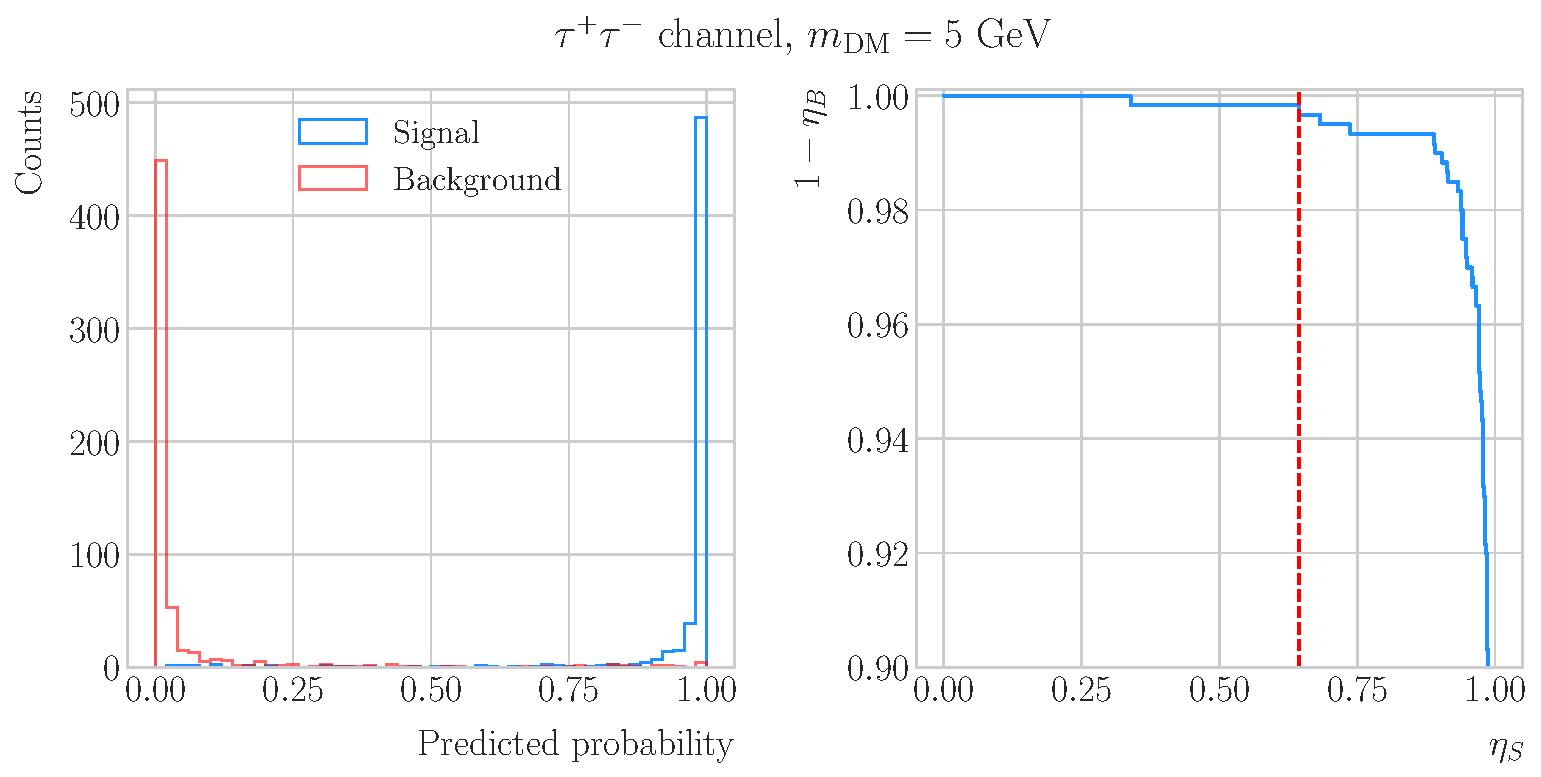
\includegraphics[width=0.95\linewidth]{Images/DM_Analysis/solardm_tau_5_qel_bdt_classifier.pdf}
	\caption[Performance of the \gls{bdt} classifier for the $\tau^{+}\tau^{-}$ \gls{qe} signal with $m_{\mathrm{DM}} = 5 \ \mathrm{GeV}$.]{Left panel: distributions of the predicted probabilities assigned by the \gls{bdt} classifier to the test sample for the signal (blue) and the atmospheric background (red). Right panel: ROC curve in the signal efficiency versus background rejection plane (blue line). The value of $\eta_{S}$ for which the target background rejection of $99.8\%$ is achieved is also indicated (dashed red line). In both cases, the signal corresponds to the $\tau^{+}\tau^{-}$ \gls{qe} sample with $m_{\mathrm{DM}} = 5 \ \mathrm{GeV}$.}
	\label{fig:solardm_tau_5_qel_classifier}
\end{figure}

Having done that, one can compute the following angular variables for our selected events:
\begin{align}
	\mathrm{cos} \ \theta_{\mu} &= \hat{p}_{\nu} \cdot \hat{p}_{\mu},\label{6.8} \\
	\mathrm{cos} \ \theta_{p} &= \hat{p}_{\nu} \cdot \hat{p}_{p},\label{6.9} \\
	\mathrm{cos} \ \theta_{N} &= \hat{p}_{\nu} \cdot \hat{p}_{N}. \label{6.10}
\end{align}

Figure \ref{fig:solardm_tau_5_qel_angular_dists} shows the distributions of these angular variables for the $\tau^{+}\tau^{-}$ \gls{qe} sample with $m_{\mathrm{DM}} = 5 \ \mathrm{GeV}$ (blue) and the atmospheric background (red). Again, for the atmospheric events I use a random solar position as the ansatz for the incoming neutrino direction. Notice that in this case the proton is typically not as forward as the hadronic jet is in the \gls{dis} events. Also, the nucleus angle is uniform for signal events, whereas for the background it is biased towards low values. However, the spread of this angular distribution is significant.

As a consequence of these features, the usual approach of applying simple angular cuts proved to be not as effective as it was in the previous situation. Therefore, as a possible solution, I tried to use a boosted decision tree (\gls{bdt}) classifier to separate between signal and background events. In this case, the predicted probability from the classification can be used to form a decision boundary, which will give an estimate of the signal efficiency and the background rejection.

For each \gls{dm} mass value and channel, as well as for the background, I divide the events into training, validation, and test samples. The input variables for the classifier are the angular variables defined in Eqs. (\ref{6.8} - \ref{6.10}). I use the \gls{bdt} classifier implemented in \texttt{scikit-learn} \cite{scikit-learn}, with a maximum depth of four trees, a maximum number of estimators of $400$, and early stopping enabled. The rest of the \gls{bdt} parameters are set to their default values. I do not perform a full optimisation of the hyperparameters, as the goal is simply to demonstrate the power of this method.

\begin{figure}[t]
	\centering
	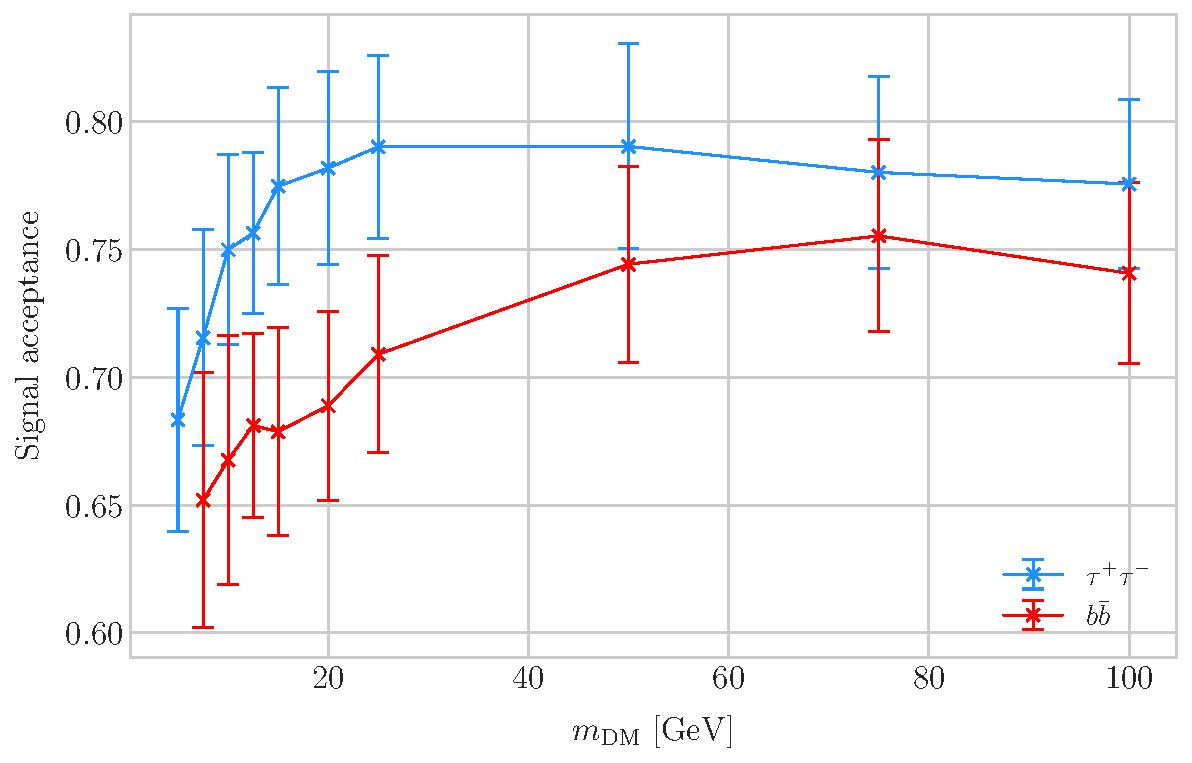
\includegraphics[width=0.9\linewidth]{Images/DM_Analysis/solardm_qel_signal_acceptance_new.pdf}
	\caption[Signal efficiencies for the $\tau^{+} \tau^{-}$ and $b\bar{b}$ single proton \gls{qe} samples as functions of the \gls{dm} mass.]{Signal efficiencies for the $\tau^{+} \tau^{-}$ (blue line) and $b\bar{b}$ (red line) single proton \gls{qe} samples as functions of the \gls{dm} mass, $m_{\mathrm{DM}}$, obtained by requiring a background rejection greater than $99.8\%$.}
	\label{fig:solardm_qel_signal_acceptance}
\end{figure}

The results of the training process for the $\tau^{+}\tau^{-}$ \gls{qe} signal with $m_{\mathrm{DM}} = 5 \ \mathrm{GeV}$ are shown in Fig. \ref{fig:solardm_tau_5_qel_classifier}. On the left panel I have the distributions of the probabilities predicted by the model, separated in true signal (blue) and background (red) events, for the test sample. On the right panel I show the receiver operating characteristic (ROC) curve for this same sample. This represents the background rejection of the classifier as a function of the signal efficiency. Requiring a background rejection of $99.80\%$ would give a signal efficiency of $64.47\%$ in this case (indicated by the dashed red line).

To obtain a robust estimate of the signal efficiencies, I use a cross-validation approach. In particular, I use the \texttt{StratifiedKFold} method in \texttt{scikit-learn}. This divides the data into $k$ equal-sized samples (or folds). Then, it performs $k$ training iterations, each time using $k-1$ of the samples as training data while the remaining fold acts as test sample. In this case, I set $k=5$ and the metric I extract from the test data is the signal efficiency value which yields a $99.80\%$ background rejection. The final signal efficiency for each channel and mass point is the mean of the metrics obtained from the cross-validation.

Figure \ref{fig:solardm_qel_signal_acceptance} shows the result of this procedure. Notice that again the efficiencies for the $\tau^{+}\tau^{-}$ channel (blue line) are consistently higher than the ones for the $b\bar{b}$ channel (red line). Similarly as before, the angular distributions of the high energy neutrinos are easier to separate from the atmospheric background. Therefore, the signal efficiency grows with the \gls{dm} mass, and benefits from a harder annihilation channel.

\begin{comment}
This can be due to the fact that, for each \gls{dm} mass point, the neutrino spectrum coming from the $b\bar{b}$ annihilation channel is centered at lower energies when compared to the $\tau^{+}\tau^{-}$ spectrum. This directly translates into more low energy neutrinos undergoing \gls{qe} interactions, which give signals that can be easily separated from the atmospheric background. This explanation also help us understand why in both cases the signal acceptance drops when the \gls{dm} mass increases. In all cases, the background rejection took values between $99.8\%$ to $99.9\%$. I will assume a $99.8\%$ background rejection value in all cases to keep our estimation conservative.
\end{comment}

\begin{figure}[t]
	\centering
	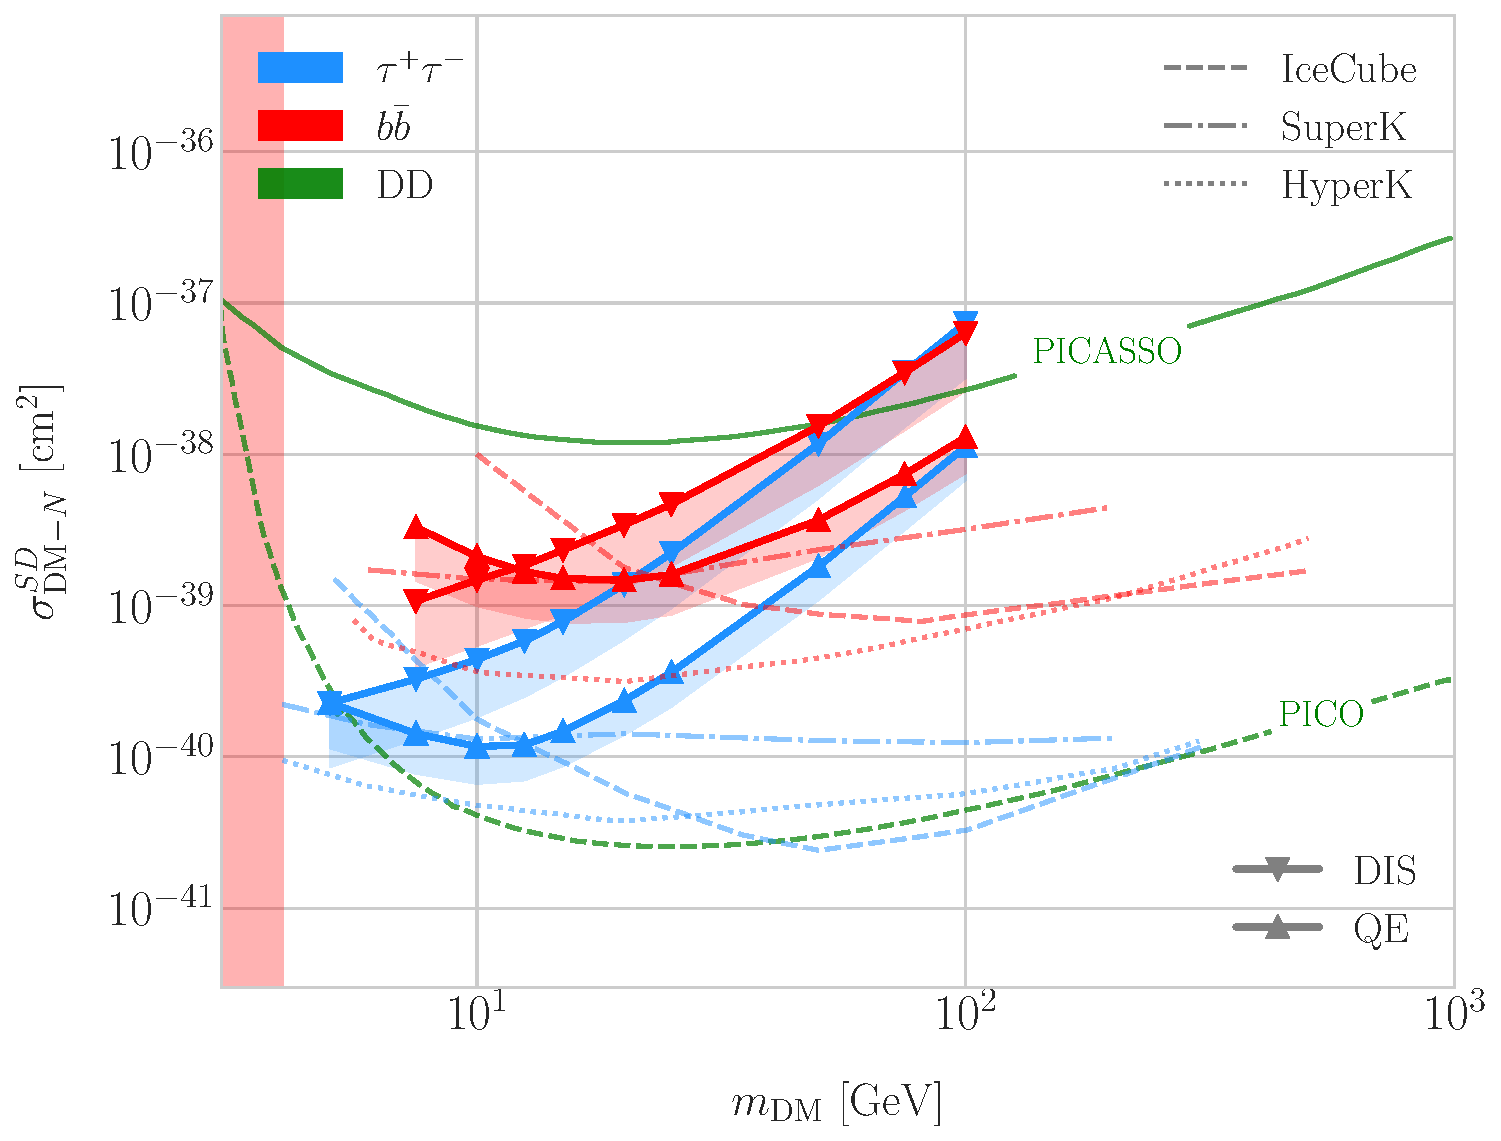
\includegraphics[width=0.95\linewidth]{Images/DM_Analysis/solardm_xsection_sd.pdf}
	\caption[Projected 90\% confidence level upper limits for \gls{dune} on the spin-dependent \gls{dm}-nucleon scattering cross section as a function of $m_{\mathrm{DM}}$.]{Projected 90\% confidence level upper limits for \gls{dune} (400 kT yr) on the spin-dependent \gls{dm}-nucleon scattering cross section as a function of $m_{\mathrm{DM}}$, for the annihilation channels $\tau^{+}\tau^{-}$ (blue) and $b\bar{b}$ (red) separated by interaction mode (up triangles denote \gls{dis} interactions whereas down triangles represent \gls{qe} interactions). I also show the previous limits from IceCube \cite{IceCube2021} (solid lines) and Super-Kamiokande \cite{Super-Kamiokande2015} (dash-dotted), and the projected sensitivities for Hyper-Kamiokande \cite{Bell2021} (dotted lines), as well as the direct detection limits from PICASSO \cite{Behnke2016} (solid green line) and PICO-60 $\mathrm{C}_{3}\mathrm{F}_{8}$ \cite{PICO2019} (dashed green line).}
	\label{fig:solardm_xsection_sd}
\end{figure}

\subsection{Results}

To estimate the \gls{dm} cross section sensitivities, the expected number of background events needs to be re-computed. As I am separating events by interaction type, Eq. (\ref{4.4}) does not hold anymore because in that case I integrated over the total neutrino-argon cross section. In this instance, the expected number of background events for \gls{dis}-like events is approximately given by:
\begin{equation}\label{6.11}
	N_{B}^{DIS} \simeq \eta_{B}^{DIS} \times \left(4.655 \times 10^{3}\right) \times \left(\frac{\mathrm{exposure}}{400 \ \mathrm{kT} \ \mathrm{yr}}\right),
\end{equation}
whereas for \gls{qe}-like events we have:
\begin{equation}\label{6.12}
	N_{B}^{QE} \simeq \eta_{B}^{QE} \times \left(2.248\times 10^{4}\right) \times \left(\frac{\mathrm{exposure}}{400 \ \mathrm{kT} \ \mathrm{yr}}\right).
\end{equation}

Now, using these together with Eqs. (\ref{4.5}) and (\ref{4.6}) one can obtain the $90\%$ C.L. upper limit on the total annihilation rate at equilibrium for both kind of events. Then, applying the computed \gls{dm}-nucleons capture rates, I can translate these into limits on the \gls{dm}-nucleon cross section by means of Eqs. (\ref{2.2}), (\ref{2.5}), and (\ref{2.6}).

Figure \ref{fig:solardm_xsection_sd} shows the obtained limits on the \gls{sd} \gls{dm}-nucleon cross section for \gls{dune}, using the \gls{dis} (up triangles) and \gls{qe} (down triangles) events both for the $\tau^{+}\tau^{-}$ (blue) and the $b\bar{b}$ (red) samples, for an exposure of $400 \ \mathrm{kT} \ \mathrm{yr}$. The coloured bands represent the difference between the realistic efficiencies obtained and the limit of perfect signal efficiency and the optimistic background rejection given by Eq. (\ref{4.3}). I also include the corresponding current limits from IceCube \cite{IceCube2021} (solid lines) and Super-Kamiokande \cite{Super-Kamiokande2015} (dash-dotted lines), as well as the projected sensitivities for Hyper-Kamiokande \cite{Bell2021} (dotted lines). For comparison, I also show the reported direct detection limits from PICASSO \cite{Behnke2016} (solid green line) and PICO-60 $\mathrm{C}_{3}\mathrm{F}_{8}$ \cite{PICO2019} (dashed green line).

Notice that, for most of the mass range, the limits one can set using the \gls{dis} events are stronger than those of the \gls{qe} interactions, except for the low mass part of both the $\tau^{+}\tau^{-}$ and the $b\bar{b}$ curves where the \gls{qe} events dominate. In general, the expected sensitivity of \gls{dune} for \gls{dm} masses $\lesssim 25 \ \mathrm{GeV}$ surpasses the stronger current indirect limits. However, experiments like Hyper-Kamiokande are foreseen to have an overall better sensitivity in this kind of searches, as they have a bigger active volume and accept a broader energy range.

A pending question is what happens when we add the \gls{res} and \gls{mec} charged-current interaction contributions. In that case, it would probably be more convenient to split the samples by final state interaction topologies. Also, another necessary improvement would be adding a full detector simulation and reconstructions. This will also require considering the effect of poorly reconstructed events or final states containing neutral particles, such that they mimic the desired topology at the reconstruction level. However, these fall out of scope for this first sensitivity study.

In Apps. \ref{sec:dm_analysis_kk_dm} and \ref{sec:dm_analysis_leptophilic_dm} I show the results of two additional studies, where I apply the techniques described before to two specific realisations of the \gls{dm} interactions (Kaluza-Klein \gls{dm} and leptophilic \gls{dm}).

\section{Systematic uncertainties}
\label{sec:dm_analysis_systematics}

The estimation of the \gls{dm} cross sections using neutrinos from \gls{wimp} annihilations inside the Sun is affected by systematic uncertainties from different sources. Surely, the atmospheric background estimation is also affected by systematic uncertainties. There are uncertainties common to both types of events, as well as others specific to each. In this section, I try to provide a comprehensive summary of the main sources of uncertainty for this analysis, which should be taken into account in any future extensions of the same.

\begin{table}[t]
	\caption[Systematic uncertainties for the solar \gls{wimp} signal events.]{Systematic uncertainties for the solar \gls{wimp} signal events. Table adapted from Ref. \cite{Principato2021}.}
	\begin{center}
		\begin{small}
			\begin{tabular}{c|c}
				Systematic                         & Value \\[2mm] \hline
				\rule{0pt}{1.1\normalbaselineskip}Form factor                      & Does not apply to \gls{sd} \cite{Wikstroem2009} \\[2mm]
				Solar model                      & $3\%$ \cite{Wikstroem2009} \\[2mm]
				Local \gls{dm} density                 & Not relevant for relative interpretations \cite{Wikstroem2009,Super-Kamiokande2015} \\[2mm]
				Dynamics of solar system         & Negligible \cite{Rott2011} \\[2mm]
				Velocity distributions           & $20\%$ at $20~\mathrm{GeV}$ \cite{Wikstroem2009,Super-Kamiokande2015} \\[2mm] \hline
				\rule{0pt}{1.1\normalbaselineskip}Oscillation parameters           & $8\%$ for $\tau^{+}\tau^{-}$, $5\%$ for $b\bar{b}$ \cite{Boliev2013} \\[2mm]
				Neutrino interactions in the Sun & $10\%$ \\[2mm]
				Matter effects in the Earth      & $10\%$ 
			\end{tabular}
		\end{small}
	\end{center}
	\label{tab:solar_dm_signal_uncertainties}
\end{table}

\subsection{Systematic uncertainties in the solar WIMP signal}

The systematic uncertainties affecting the solar \gls{wimp} neutrino signal can be divided in two categories. On the one hand, we have those affecting the solar \gls{wimp} annihilation rate. On the other hand, there are the ones which modify the neutrino flux resulting from the annihilations reaching our detector.

\begin{itemize}
	\item \textbf{Uncertainties on the annihilation rate}. These include the astrophysical effects that affect the normalisation of the solar \gls{dm} neutrino flux. The main contributions are the solar model choice, the form factor uncertainties (only for \gls{si} searches), the gravitational effect of other planets, the local \gls{dm} density (not relevant for relative comparisons, as it affects direct detection experiments in the same way), and the \gls{dm} halo and dispersion velocities.
	\item \textbf{Uncertainties on the neutrino flux}. These are related to the oscillation effects, as well as the absorption and regeneration of neutrinos in the Sun. Matter effects inside the Earth also affect the neutrino flux measured by the detectors.
\end{itemize}

Table \ref{tab:solar_dm_signal_uncertainties} summarises the contributions of the different sources of uncertainty for the signal events. These are the signal systematic uncertainties that have been taken into account in previous solar \gls{dm} searches with neutrinos \cite{Boliev2013,Super-Kamiokande2015,Principato2021}.

\begin{table}[t]
	\caption[Systematic uncertainties for the solar \gls{wimp} atmospheric background events.]{Systematic uncertainties for the solar \gls{wimp} atmospheric background events. Table adapted from Ref. \cite{Super-Kamiokande2017}.}
	\begin{center}
		\begin{small}
			\begin{tabular}{c|c}
				Systematic                                            & Value \\[2mm] \hline
				\rule{0pt}{1.1\normalbaselineskip}Flux normalisation                                    & $25-7\%$ for $0.1 < E_{\nu} \leq 1~\mathrm{GeV}$ (linear in $\mathrm{log} ~ E_{\nu}$)\\[1mm] & $7\%$ up to $10~\mathrm{GeV}$ \\[2mm]
				$(\nu_{\mu}+\bar{\nu}_{\mu})/(\nu_{e}+\bar{\nu}_{e})$ & $2\%$ for $E_{\nu} \leq 1~\mathrm{GeV}$ \\[1mm] & $3\%$ for $1 < E_{\nu} \leq 10~\mathrm{GeV}$ \\[2mm]
				$\bar{\nu}_{\mu}/\nu_{\mu}$                           & $2\%$ for $E_{\nu} \leq 1~\mathrm{GeV}$ \\[1mm] & $6\%$ for $1 < E_{\nu} \leq 10~\mathrm{GeV}$ \\[2mm]
				$\mathrm{K}/\pi$ ratio                                & $5\%$ $E_{\nu} \leq 100~\mathrm{GeV}$
			\end{tabular}
		\end{small}
	\end{center}
	\label{tab:solar_dm_background_uncertainties}
\end{table}

\subsection{Systematic uncertainties in the atmospheric background}

For the atmospheric background events, one needs to take into account the systematic uncertainties affecting the atmospheric $\nu_{\mu}$ flux. These have been extensively studied in the context of atmospheric neutrino oscillation measurements. Among these, the energy-dependent flux normalisation uncertainty dominates in the low energy regime. Other important contributions to the uncertainty come from the ratios between the muon to electron neutrino and the muon to anti-muon neutrino components of the flux. Additional uncertainty is introduced by the errors in the pion and kaon production rates calculated for the hadronic interactions of cosmic rays in the atmosphere \cite{Honda2006}.

Table \ref{tab:solar_dm_background_uncertainties} shows a summary of the leading contributions to the uncertainty on the atmospheric muon neutrino flux, in the energy range relevant for this analysis.

\subsection{Common systematic uncertainties}

Finally, there are sources of uncertainty common to both signal and backgrounds. These have two different origins:

\begin{itemize}
	\item \textbf{Uncertainties on the neutrino cross section}. These are introduced by the modelling of the neutrino-nucleus interactions. In the context of the solar \gls{wimp} analysis, these have been estimated to be $10\%$ for \gls{dm} masses around $10~\mathrm{GeV}$ \cite{Boliev2013}.
	\item \textbf{Uncertainties related to the detector}. They affect the measurement of the neutrino interaction and the final state particles produced. The main detector uncertainties relevant to this analysis are those related to the energy and angular resolutions of the \gls{dune} \gls{fd}. Other effects, like the timing and triggering efficiencies, will also contribute to the uncertainties. The particular values these will take for this analysis need to be evaluated in the context of \gls{dune}.
\end{itemize}

In this Chapter, I discussed my work on the solar \gls{dm} analysis. Here I explain how the \gls{dune} \gls{fd} can be used to probe \gls{dm} interactions by measuring the neutrino flux coming from \gls{dm} annihilations in the core of the Sun. After introducing the topic of \gls{dm} capture and annihilation in a massive object like the Sun in section \ref{sec:dm_analysis_theory}, I describe what kind of neutrino signals one can expect from such events in section \ref{sec:dm_analysis_flux}. Later, in section \ref{sec:dm_analysis_limits} I comment on how \gls{dune} could constrain the \gls{dm} parameter space by performing counting experiments. In section \ref{sec:dm_analysis_high_e_nu} I study the selection efficiency for the $\tau^{+}\tau^{-}$ and $b\bar{b}$ channels. I focus on two different kinematic regimes: the high energy neutrinos where \gls{dis} interactions with argon dominate, and the low energy part of the spectrum where neutrinos mainly undergo \gls{qe} interactions. This allows me to compute the projected generator-level \gls{dm} cross section sensitivities, showing how \gls{dune} can be complementary to other indirect \gls{dm} searches. Additionally, I present a summary of the relevant systematic uncertainties in section \ref{sec:dm_analysis_systematics}.